\documentclass[11pt, a4paper]{article}
\documentclass[a4paper,12pt]{report}

%\usepackage{showframe}
\usepackage[utf8]{luainputenc}

\usepackage[a4paper, margin=1in]{geometry}

\usepackage{float}
\usepackage{textcomp}
\usepackage{amstext}
\usepackage{graphicx}
\usepackage[spanish]{babel}
\usepackage{tikz}
\usepackage[american, oldvoltagedirection]{circuitikz}
\usepackage{amsmath}
\usepackage{siunitx}

\usepackage{pgfplots}
\pgfplotsset{width=10cm, compat=1.9}

\usepackage{relsize}

\begin{document}

\part{Celda Sallen-Key} 
\section{Introducción}
	Se llama filtros activos a aquellos que agregan componentes activos al circuito, como lo es en este caso la utilización de un amplificador operacional. En el caso de la celda Sallen-Key se utilizan solo resistores y capacitores como componentes pasivos y dependiendo de su ubicación dentro del circuito se obtienen los diferentes tipos de filtros.
	En esta primer parte se mostrará el análisis e implementación de celdas Sallen-Key para la creación de dos filtros pasa-bajos, utilizando la aproximación de Legendre para uno y la de Bessel para el restante.
	
\begin{figure}[H]
	\centering
	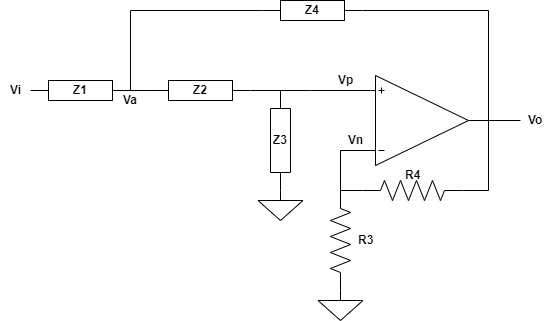
\includegraphics[scale=0.5]{sallenkeygenerico.jpg}
	\caption{Celda Sallen-Key genérica}
	\label{fig:sallenkeygenerica}
\end{figure}
	
\section{Análisis Teórico}

\subsubsection{Función Transferencia}
	A continuación en esta sección se realizará el análisis del circuito, se buscará la función transferencia genérica y luego se harán los reemplazos necesarios para obtener la del filtro pasa-bajos.
	
\begin{equation}
	\begin{cases}	
			V_o = A_{Vol} \, (Vp - Vn) \\
			V_o = V_n \, K \\
			V_p = Va \, \frac{Z_3}{Z_2 + Z_3} \\
			\dfrac{V_a - V_{in}}{Z_1} + \dfrac{V_a - V_p}{Z_2} + \dfrac{V_a - V_o}{Z_4} = 0		
	\end{cases}
\end{equation}

Donde $K = \dfrac{R_3 + R_4}{R_3}$. Utilizando software de cálculo y la aproximación de $A_{Vol}$ infinito se obtiene la siguiente expresión:

\begin{equation}
	H(S) = \dfrac{V_o}{V_{in}} =\dfrac{K}{\dfrac{Z_1 \, Z_2}{Z_3 \, Z_4} + \dfrac{Z_1 + Z_2}{Z_3} + \dfrac{Z_1 \, (1-K)}{Z_4} + 1}	
\end{equation}

\begin{figure}[H]
	\centering
	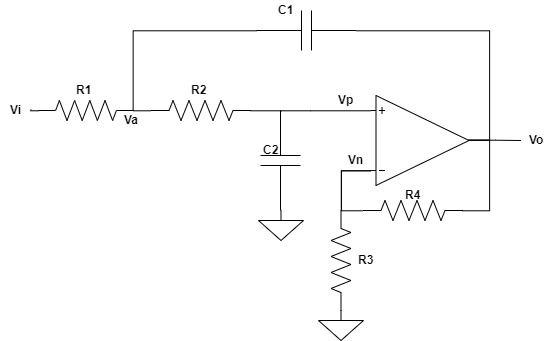
\includegraphics[scale=0.5]{sallenkeypasabajos.jpg}
	\caption{Celda Sallen-Key genérica}
	\label{fig:sallenkeypasabajos}
\end{figure}
	
	Para el caso de un filtro pasa-bajos se cambias las impedancias por resistencias y capacitores de la forma que puede observarse en la Figura \ref{fig:sallenkeypasabajos} y se obtiene la función transferencia siguiente:

\begin{equation}
		H(S) = \dfrac{K}{(R_1 \, R_2 \, C_1 \, C_2) \, S^2 + ( \,(R_1 + R_2) C_2 + (1-K)C_1 \, R_1) S +1}
\end{equation}

\begin{equation} 
	H(S) = \dfrac{1+ \dfrac{R_4}{R_3}}{\left(R_1 \, R_2 \, C_1 \, C_2 \right) \, S^2 + \left( \, \left(R_1 + R_2 \right) C_2 - C_1 \, R_1 \, \dfrac{R_4}{R_3} \right) S +1}	
	\label{eq:transfpasabajos}
\end{equation}
	
	Habiendo reemplazado $Z_1 = R_1 \, , \, Z_2 = R_2 \, , \, Z_3 = \dfrac{1}{S \, C_2} \, , \, Z_4 = \dfrac{1}{S \, C_1}$. 
	Se puede despejar de la Ecuación \ref{eq:transfpasabajos} que:

\begin{equation}
W_0 = \dfrac{1}{\sqrt[]{R_1 \, R_2 \, C_1 \, C_2}}
	\label{eq:freqdecorte}
\end{equation}	

\begin{equation}
\dfrac{\sqrt[]{R_1 \, R_2 \, C_1 \, C_2}}{R_1 \, (C_1 + C_2) - R_2 \, C_2 \, \dfrac{R_4}{R_3}}
	\label{eq:Q}
\end{equation}

\subsubsection{Sensibilidades}

%Se parecen a las de Marce

\begin{table}[H]
\centering
\begin{tabular}{|c|c|c|}
\hline
\multicolumn{3}{|c|}{\textbf{Celda Sallen-Key}} 	\\ \hline
               & $\mathbf{W_0}$  & $\mathbf{Q}$   	\\ \hline
$R_1$             & -1/2           & $\frac{1}{2} \, \frac{C_1 
\, R_1 \, R_4 + R_3 \, C_2 \, R_2 - R_3 \, C_2 \, R_1}{(C_2 \, R_3 \, (R_1+R_2)- C_1 \, R_1 \, R_4}$            \\ \hline
$R_2$             & -1/2            & $- \frac{1}{2} \, \frac{C_1 
\, R_1 \, R_4 + R_3 \, C_2 \, R_2 - R_3 \, C_2 \, R_1}{C_2 \, R_3 \, (R_1+R_2)- C_1 \, R_1 \, R_4}$            \\ \hline
$C_1$             & -1/2            & $- \frac{1}{2} \, \frac{C_1 \, R_1 \, R_4 + C_2 \, (R_1+R_2)}{C_1 \, R_1 \, R_4 - C_2 \, R_3 \,(R_1+R_2)}$            	\\ \hline
$C_2$             & -1/2            & $\frac{1}{2} \, \frac{C_1 \, R_1 \, R_4 + C_2 \, (R_1+R_2)}{C_1 \, R_1 \, R_4 - C_2 \, R_3 \,(R_1+R_2)}$            	\\ \hline
$R_3$             & 0               & $\frac{C_1 \, R_1 \, R_4}{C_1 \, R_1 \, R_4 - C_2 \, R_3 \, (R1+R2)}$            \\ \hline
$R_4$             & 0               & $- \, \frac{C_1 \, R_1 \, R_4}{C_1 \, R_1 \, R_4 - C_2 \, R_3 \, (R1+R2)}$            \\ \hline
\end{tabular}
\end{table}

	Se puede observar que $W_0$ es de igual forma sensible tanto a $R_1 \, R_2 \, C_1$ y $C_2$, mientras que $Q$ depende de los componentes elegidos.
	
\section{Diseño del Filtro}

	Se busca implementar dos filtros pasa-bajos con las siguientes características:
\begin{table}[H]
\centering
\begin{tabular}{|c|c|}
\hline
\multicolumn{2}{|c|}{\textbf{Legendre}} \\ \hline
$\mathbf{Orden}$        & $5$             \\ \hline
$\mathbf{f_p}$          & $33 \, kHz \pm 5 \% $          \\ \hline
$\mathbf{A_p}$          & $3 \, dB$          \\ \hline
$\mathbf{|Z_{in}(f)|}$  & $ \geq \SI{50}{k\ohm}$          \\ \hline
\end{tabular}
\caption{Legendre para alta señal}
\label{tabla:legendre}
\end{table}

\begin{table}[H]
\centering
\begin{tabular}{|c|c|}
\hline
\multicolumn{2}{|c|}{\textbf{Bessel}} \\ \hline
$\mathbf{f_p}$           & $2200 \, Hz$             \\ \hline
$\mathbf{f_a}$           & $10400 \, Hz$          \\ \hline
$\mathbf{A_p}$           & $3 \, dB$          \\ \hline
$\mathbf{Aa}$           & $40 \, dB$          \\ \hline
$\mathbf{\Upsilon(f_p)}$           & $\leq 5 \, \% $             \\ \hline
$\mathbf{|Z_{in}(f)|}$          & $\geq \SI{50}{k\ohm}$             \\ \hline
\end{tabular}
\caption{Bessel para baja señal}
\label{tabla:bessel}
\end{table}

\subsection{Legendre}

	Mediante el empleo de software se logró conseguir la función transferencia del circuito mediante la aproximación por polinomios de Legendre y como resultado se obtuvo:
	
\begin{equation}
	H(S) = \dfrac{G}{(s+p_1)(s+p_1^*)(s+p_2)(s+p_2^*)(s+p3)}
\label{eq:legendrepolos}
\end{equation}

	Con los valores $p_1 = (-32840 + 206900 \, j ) \, , \, p_2 = (-82990 + 125800 \, j) \, , \, y p_3 = -100100$, se puede notar que se necesita de tres etapas, una de primer orden y otras dos de segundo orden.
	Para las dos etapas de orden dos se utilizarán dos celdas Sallen-Key con la configuración pasa-bajos. A partir de la Ecuación \ref{eq:legendrepolos} podemos obtener:
	
\begin{equation}
{W_0}_1 = 209.5 \, k \frac{rad}{s}
\label{eq:wo1Legendre}
\end{equation}

\begin{equation}
Q_1 = 3.19
\label{eq:Q1Legendre}
\end{equation}

\begin{equation}
{W_0}_2 = 1.51 \, k \frac{rad}{s}
\label{eq:wo2Legendre}
\end{equation}

\begin{equation}
Q_2 = 0.91
\label{eq:Q2Legendre}
\end{equation}

	Para la etapa de orden uno se eligió usar un circuito integrador compensado y a partir de la Ecuación \eqref{eq:legendrepolos} se sabe que ${W_0}_3 = 100.1 \, kHz$ y $Q_3 = 0.5$.
	
\begin{figure}[H]
	\centering
	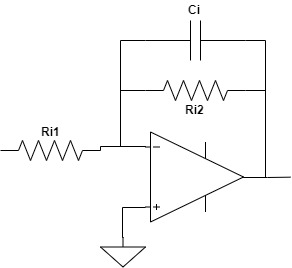
\includegraphics[scale=0.5]{integradorcompensado.jpg}
	\caption{Circuito integrador compensado}
	\label{fig:sallenkeypasabajos}
\end{figure}
	
	Entonces se eligieron los siguientes valores de componentes:
	
\begin{table}[H]
\centering
\begin{tabular}{|c|c|c|}
\hline
            & \textbf{Etapa 1} & \textbf{Etapa 2} \\ \hline
$\mathbf{R_1}$ & $\SI{26}{\ohm}$               & $\SI{7.7}{k\ohm}$             \\ \hline
$\mathbf{R_2}$ & $\SI{26}{\ohm}$               & $\SI{7.7}{k\ohm}$             \\ \hline
$\mathbf{C_1}$ & $470 \, nF$             & $4.1 \, nF$              \\ \hline
$\mathbf{C_2}$ & $142.6 \, nF$           & $100 \, pF$             \\ \hline
$\mathbf{R_3}$ & $\SI{4.7}{M\ohm}$             & $\SI{4.7}{M\ohm}$             \\ \hline
$\mathbf{R_4}$ & $\SI{77.6}{\ohm}$             & $\SI{77.6}{\ohm}$             \\ \hline
\end{tabular}
\caption{Valores de componentes para etapas de orden dos}
\label{tabla:legendreetapasorden2}
\end{table}

\begin{table}[H]
\centering
\begin{tabular}{|c|c|c|}
\hline
$\mathbf{Ri1}$ & $\mathbf{Ri2}$ & $\mathbf{Ci}$     \\ \hline
$\mathbf{\SI{56}{k\ohm}}$ & $\mathbf{\SI{56}{k\ohm}}$ & $\mathbf{183.8 \,pF}$ \\ \hline
\end{tabular}
\caption{Valores de componentes para la etapa de orden uno}
\label{tabla:legendreetapaorden1}
\end{table}
	Algunos valores al no ser comerciales se busca obtenerlos mediante combinación de otros valores.
	El orden de etapas se eligió teniendo en cuenta la selectividad de cada etapa del circuito, como se desea trabajar con alta señal se ordenaron de manera de maximizar el rango dinámico del filtro, teniendo así en primera posición aquella que presenta menor sobrepico, esto es importante para evitar un incremento de tension a la salida que podría saturar las demás etapas.
\begin{figure}[H]
	\centering
	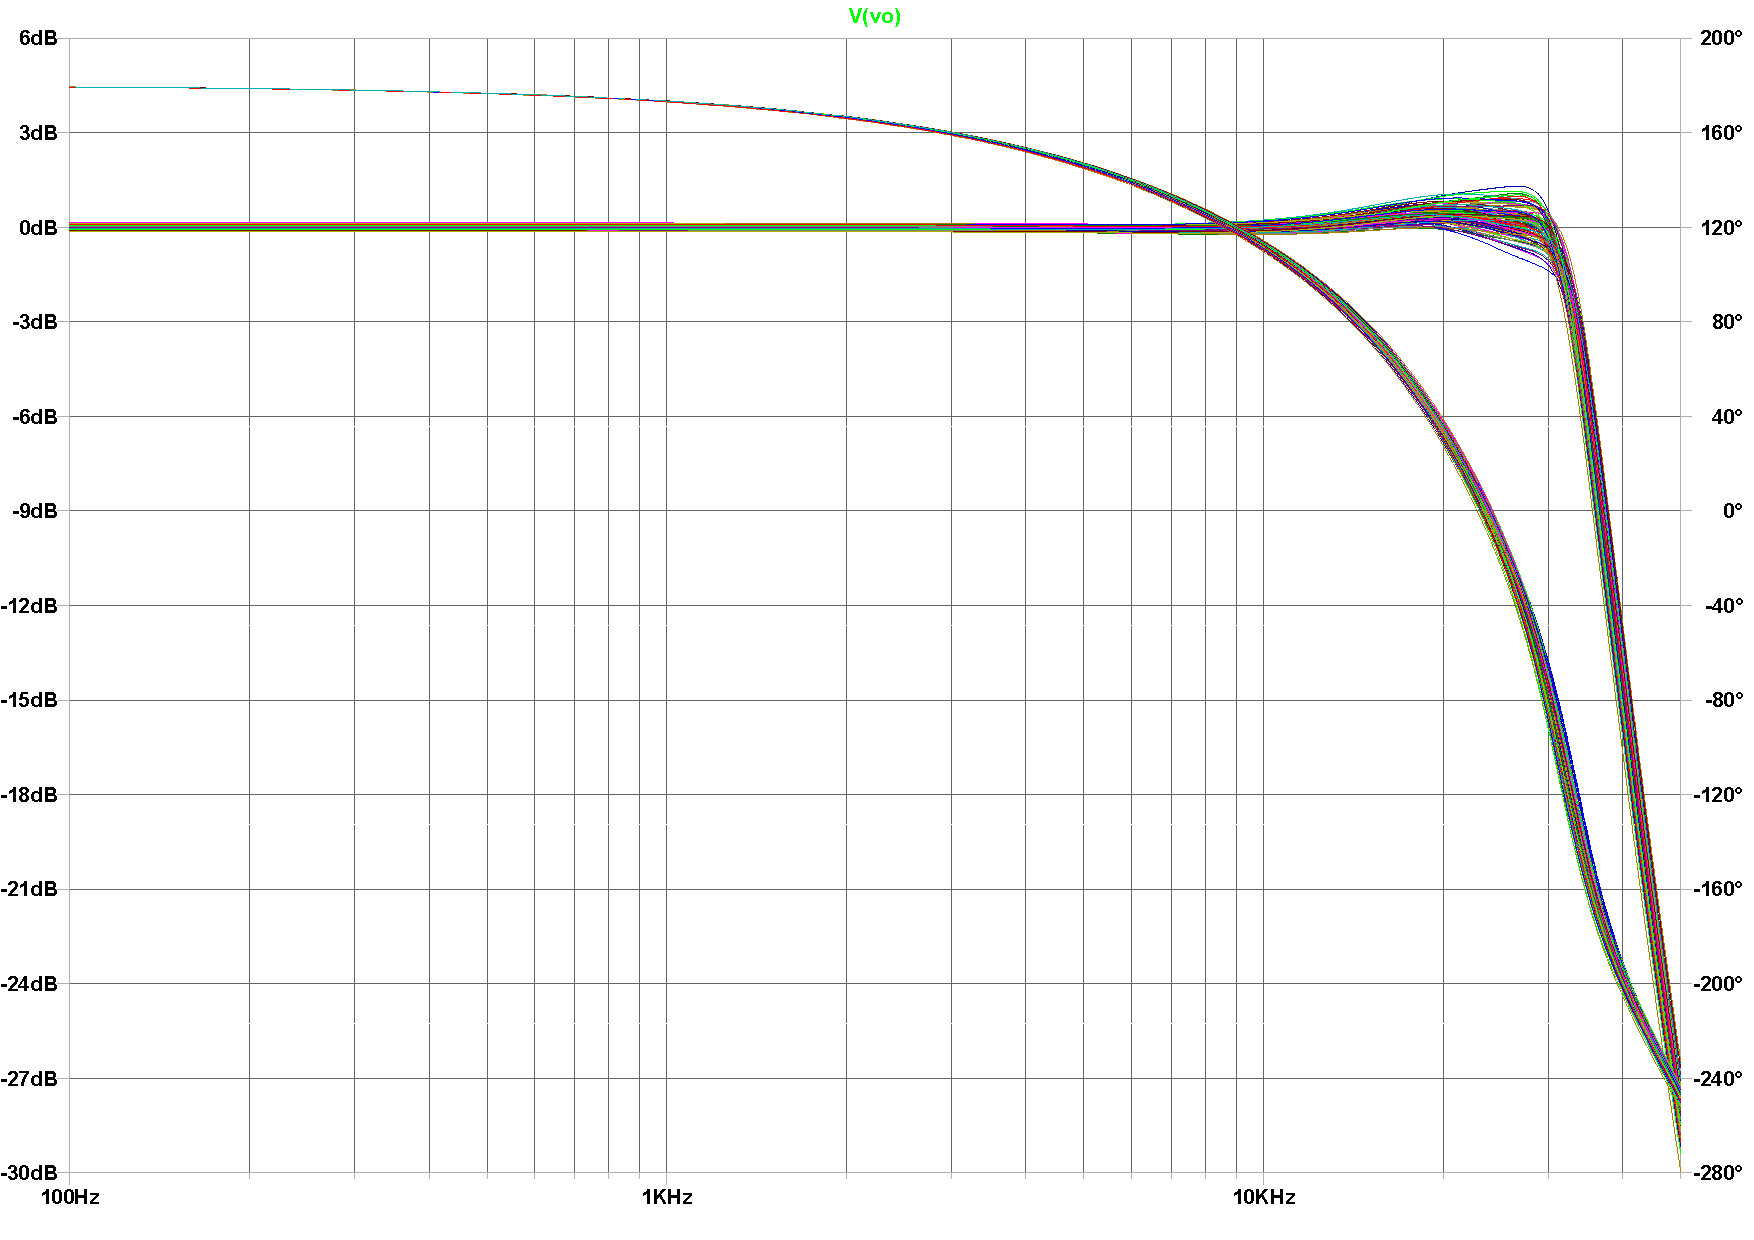
\includegraphics[scale=0.5]{montecarlolegendre.pdf}
	\caption{Montecarlo con los componentes elegidos}
	\label{fig:montecarlolegendre}
\end{figure}
	En este diagrama de montecarlo se puede observar que al momento en que la atenuación es de $3 \, dB$, el peor caso hacia ambos extremos cae dentro del margen del $\pm 5 \%$ que se especifica de $f_p = 33 \, kHz$.

\subsection{Bessel}
	De igual manera que con el caso de la aproximación anterior se consiguió obtener la funcion transferencia que resulto ser la siguiente:

\begin{equation}
	H(S) = \dfrac{G}{(s+p_1)(s+p_1^*)(s+p_2)(s+p_2^*)(s+p3)}
\label{eq:besselpolos}
\end{equation}

	Con $p_1 = -13260 + 20370 \, j$ , $p_2 = -19120 + 9940 \,j$ y $p_3 = -20800$.
	Se utilizo la misma configuración que para el caso anterior solo que se cambio el orden, ahora colocando en primer lugar aquella con mayor $Q$ ya que al ser para baja señal no queremos que se atenúe demasiado y se pueda mezclar con el piso de ruido.
	De la Ecuación \eqref{eq:besselpolos} se consiguen los siguientes valores:

\begin{equation}
	{W_0}_1 = 24.3 \, kHz
\label{eq:wo1Bessel}
\end{equation}

\begin{equation}
	Q_1 = 0.92
\end{equation}

\begin{equation}
	{W_0}_2 = 21.55 \, kHz
\end{equation}

\begin{equation}
	Q_2 = 0.56
\end{equation}

	Estos primeros fueron para las etapas de orden dos y a continuación lo conseguido para la de orden uno.

\begin{equation}
	{W_0}_3 = 20800 \, kHz
\end{equation}

\begin{equation}
	Q_3 = 0.5
\end{equation}

	Gracias a esto se consiguieron los siguientes valores de componentes:
\begin{table}[H]
\centering
\begin{tabular}{|c|c|c|}
\hline
            & \textbf{Etapa 1} & \textbf{Etapa 2} \\ \hline
$\mathbf{R_1}$ & $\SI{100}{k\ohm}$               & $\SI{7.7}{k\ohm}$             \\ \hline
$\mathbf{R_2}$ & $\SI{100}{k\ohm}$               & $\SI{7.7}{k\ohm}$             \\ \hline
$\mathbf{C_1}$ & $754.2 \, pF$             & $523 \, pF$              \\ \hline
$\mathbf{C_2}$ & $224.5 \, pF$           & $411.8 \, pF$             \\ \hline
$\mathbf{R_3}$ & $\SI{2.2}{M\ohm}$             & $\SI{2.2}{M\ohm}$             \\ \hline
$\mathbf{R_4}$ & $\SI{24}{\ohm}$             & $\SI{24}{\ohm}$             \\ \hline
\end{tabular}
\caption{Valores de componentes para etapas de orden dos}
\label{tabla:legendreetapasorden2}
\end{table}

	Estos valores mediante combinaciones se pueden conseguir con un error menor al $1 \%$.
	


\end{document}